%%%%%%%%%%%%%%%%%%%%%%%%%%%%%%%%%%%%%%%%%
% Wenneker Assignment
% LaTeX Template
% Version 2.0 (12/1/2019)
%
% This template originates from:
% http://www.LaTeXTemplates.com
%
% Authors:
% Vel (vel@LaTeXTemplates.com)
% Frits Wenneker
%
% License:
% CC BY-NC-SA 3.0 (http://creativecommons.org/licenses/by-nc-sa/3.0/)
% 
%%%%%%%%%%%%%%%%%%%%%%%%%%%%%%%%%%%%%%%%%

%----------------------------file:///home/thiago/Documentos/NLP/TP1/word2vec/trunk/datasets/results.png------------------------------------------------------------
%	PACKAGES AND OTHER DOCUMENT CONFIGURATIONS
%----------------------------------------------------------------------------------------

\documentclass[11pt]{scrartcl} % Font size
\usepackage{float}
\usepackage{hyperref}
%%%%%%%%%%%%%%%%%%%%%%%%%%%%%%%%%%%%%%%%%
% Wenneker Assignment
% Structure Specification File
% Version 2.0 (12/1/2019)
%
% This template originates from:
% http://www.LaTeXTemplates.com
%
% Authors:
% Vel (vel@LaTeXTemplates.com)
% Frits Wenneker
%
% License:
% CC BY-NC-SA 3.0 (http://creativecommons.org/licenses/by-nc-sa/3.0/)
% 
%%%%%%%%%%%%%%%%%%%%%%%%%%%%%%%%%%%%%%%%%

%----------------------------------------------------------------------------------------
%	PACKAGES AND OTHER DOCUMENT CONFIGURATIONS
%----------------------------------------------------------------------------------------

\usepackage{amsmath, amsfonts, amsthm} % Math packages

\usepackage{listings} % Code listings, with syntax highlighting

\usepackage[english]{babel} % English language hyphenation

\usepackage{graphicx} % Required for inserting images
\graphicspath{{Figures/}{./}} % Specifies where to look for included images (trailing slash required)

\usepackage{booktabs} % Required for better horizontal rules in tables

\numberwithin{equation}{section} % Number equations within sections (i.e. 1.1, 1.2, 2.1, 2.2 instead of 1, 2, 3, 4)
\numberwithin{figure}{section} % Number figures within sections (i.e. 1.1, 1.2, 2.1, 2.2 instead of 1, 2, 3, 4)
\numberwithin{table}{section} % Number tables within sections (i.e. 1.1, 1.2, 2.1, 2.2 instead of 1, 2, 3, 4)

\setlength\parindent{0pt} % Removes all indentation from paragraphs

\usepackage{enumitem} % Required for list customisation
\setlist{noitemsep} % No spacing between list items

%----------------------------------------------------------------------------------------
%	DOCUMENT MARGINS
%----------------------------------------------------------------------------------------

\usepackage{geometry} % Required for adjusting page dimensions and margins

\geometry{
	paper=a4paper, % Paper size, change to letterpaper for US letter size
	top=2.5cm, % Top margin
	bottom=3cm, % Bottom margin
	left=3cm, % Left margin
	right=3cm, % Right margin
	headheight=0.75cm, % Header height
	footskip=1.5cm, % Space from the bottom margin to the baseline of the footer
	headsep=0.75cm, % Space from the top margin to the baseline of the header
	%showframe, % Uncomment to show how the type block is set on the page
}

%----------------------------------------------------------------------------------------
%	FONTS
%----------------------------------------------------------------------------------------

\usepackage[utf8]{inputenc} % Required for inputting international characters
\usepackage[T1]{fontenc} % Use 8-bit encoding


%----------------------------------------------------------------------------------------
%	SECTION TITLES
%----------------------------------------------------------------------------------------

\usepackage{sectsty} % Allows customising section commands

\sectionfont{\vspace{6pt}\centering\normalfont\scshape} % \section{} styling
\subsectionfont{\normalfont\bfseries} % \subsection{} styling
\subsubsectionfont{\normalfont\itshape} % \subsubsection{} styling
\paragraphfont{\normalfont\scshape} % \paragraph{} styling

%----------------------------------------------------------------------------------------
%	HEADERS AND FOOTERS
%----------------------------------------------------------------------------------------

\usepackage{scrlayer-scrpage} % Required for customising headers and footers

\ohead*{} % Right header
\ihead*{} % Left header
\chead*{} % Centre header

\ofoot*{} % Right footer
\ifoot*{} % Left footer
\cfoot*{\pagemark} % Centre footer
 % Include the file specifying the document structure and custom commands

%----------------------------------------------------------------------------------------
%	TITLE SECTION
%----------------------------------------------------------------------------------------

\title{	
	\normalfont\normalsize
	\textsc{Departamento de Ciência da Computaçao - UFMG}\\ % Your university, school and/or department name(s)
	\vspace{25pt} % Whitespace
	\rule{\linewidth}{0.5pt}\\ % Thin top horizontal rule
	\vspace{20pt} % Whitespace
	{\huge Trabalho Prático I - Aprendizado Profundo para Processamento de Linguagem Natural}\\ % The assignment title
	\vspace{12pt} % Whitespace
	\rule{\linewidth}{2pt}\\ % Thick bottom horizontal rule
	\vspace{12pt} % Whitespace
}

\author{\LARGE Thiago Malta Coutinho\\ thiagomaltac@gmail.com} % Your name

\date{\normalsize\today} % Today's date (\today) or a custom date

\begin{document}



\maketitle % Print the title

%----------------------------------------------------------------------------------------
%	FIGURE EXAMPLE
%----------------------------------------------------------------------------------------

\section{Introdução}

O objetivo desse trabalho prático é estudar o funcionamento do modelo de linguagem \textbf{Word2Vec} e explorar como os métodos \textbf{CBOW} e \textbf{Skip-gram} se comportam com a variação do tamanho da janela e do corpus. Para avaliar os resultados a similaridade de cossenos foi utilizada.

\begin{figure}[h] % [h] forces the figure to be output where it is defined in the code (it suppresses floating)
	\centering
	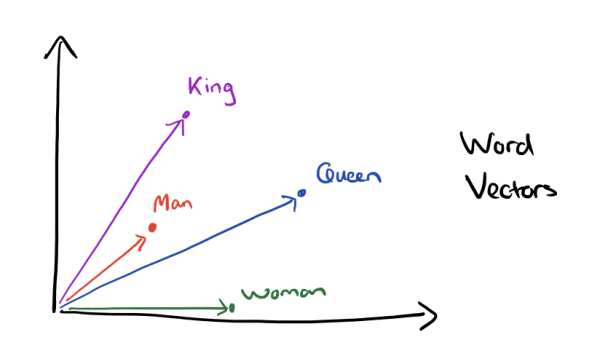
\includegraphics[width=0.5\columnwidth]{./Figures/word2vec.png} % Example image
	\caption{Representação das palavras como vetores.}
\end{figure}

%------------------------------------------------

\subsection{Word2Vec}

O modelo de linguagem \textit{Word2Vec} trouxe grandes avanços em relação aos modelos de linguagem frequentistas, gerando representações das palavras que podem servir de entrada para outros modelos de aprendizado ou produzir resultados a partir da distância do cosseno. Ele utiliza uma rede neural com uma camada de neurônios sem função não-linear em sua saída, as palavras são as entradas e saídas da rede e são codificadas em formato \textit{one-hot}; caso exista mais de uma palavra na entrada ou na saída, os vetores \textit{one-hot} são concatenados. A rede projeta os vetores codificados em uma dimensão de tamanho igual número de neurônios e otimiza os pesos da projeção com o objetivo de minimizar a função de custo presente na saída. A função de custo utilizada geralmente é a log-verossimilhança, atualizada com o algoritmo \textit{Backpropagation}, e as probabilidades de cada classe(palavra) são estimadas utilizando a função \textit{Softmax} logo após a saída da camada escondida.tempo
Uma característica importante do algoritmo é a modelagem do contexto em que as palavras aparecem, podendo ser feita de duas formas: utilizando o \textit{CBOW} ou  \textit{Skip-gram}, técnicas que serão apresentados nas Seções \ref{sec:cbow} e \ref{sec:skipgram}.

\begin{figure}[H] % [h] forces the figure to be output where it is defined in the code (it suppresses floating)
	\centering
	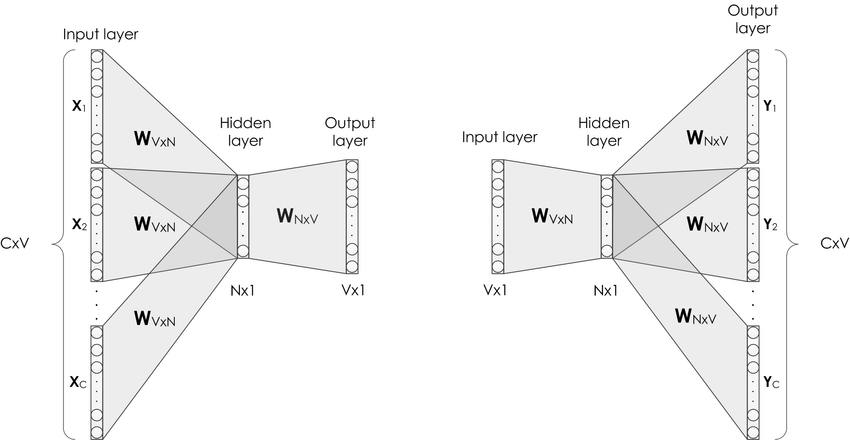
\includegraphics[width=0.7\columnwidth]{./Figures/cbow_skip.png} % Example image
	\caption{Estrutura do \textit{Word2Vec} utilizando o \textit{CBOW}(esquerda) e \textit{Skip-gram}(direita).}
\end{figure}


\subsubsection{CBOW}\label{sec:cbow}

A abordagem \textit{Continuous bag of words}(CBOW) é uma das técnicas utilizadas para modelar contexto. Nessa técnica, dado uma janela de contexto, a palavra central é a palavra a ser predita e as palavras restantes constituem o contexto linguístico atual.

\subsubsection{Skip-gram}\label{sec:skipgram}

O Skip-gram funciona de forma análoga ao CBOW, dado uma janela de contexto a palavra central é a entrada e o restante das palavras são a saída da rede.
\subsubsection{Similaridade de Cossenos}

Os vetores gerados pelo modelo podem ser normalizados para possuírem norma unitária, pertencendo à casca de uma hiper-esfera n-dimensional, onde n é o tamanho da camada escondida. Para comparar vetores, a distância euclidiana se mostra pouco eficaz e a Similaridade de Cossenos se mostra mais apropriada. A Similaridade mede o quão dois vetores estão próximos, sua fórmula é apresentada a seguir:

\begin{equation}
cos_{similarity} = \frac{\sum{(a-b)^{2}}}{\sqrt{\sum{a^{2}}}\cdot\sqrt{\sum{b^{2}}}}
\end{equation}

Onde \texttt{a} e \texttt{b} são vetores. 	
	
\section{Experimento}

A implementação utilizada para os experimento é o algoritmo desenvolvido pelo o Google em linguagem C, disponível no link \hyperlink{Word2Vec(Google)}{https://code.google.com/archive/p/word2vec/}. Também foram desenvolvidas funções auxiliares em linguagem \texttt{python} e \texttt{shell} para processamento dos dados, treinamento dos modelos e processamento dos resultados.

A metodologia consiste em treinar um modelo de linguagem para cada conjunto de hiper-parâmetros especificados na Seção \ref{sec:hiperparams}. A avaliação de desempenho dos modelos é feita utilizando o arquivo \texttt{word-analogies.txt} para gerar analogias com cada modelo treinado e comparar a palavra predita com a analogia correta, a comparação é feita com a Similaridade de Cossenos. O resultado final é a média de Similaridade.

Foi necessário fazer modificações nos arquivos \texttt{word-analogy.c} e \texttt{distance.c} para que as entradas fossem lidas de arquivos gerados por códigos intermediários em linguagem \texttt{python} e as saídas fossem formatadas de maneira a facilitar o experimento.

\subsection{Corpus}
O conjunto de dados de entrada do treinamento foi o \textit{text8}, disponível no link\\ \hyperlink{corpus(text8)}{https://mattmahoney.net/dc/text8.zip}. O Corpus tem tamanho de 95.4MiB e contém 17.005.207 palavras, não possui  pontuação e com algumas normalizações de texto aplicadas.

\subsection{Pré-processamento}

O pré-processamento dos dados foi feito com o auxílio da biblioteca \texttt{gensim}, em linguagem \texttt{python}. 
Palavras de tamanho menor que 3 foram retiradas com a função \texttt{strip\_short}, as \textit{stop-words} foram removidas chamando a função \texttt{remove\_stopwords} e por fim os números entre 0 e 9(\textit{one, two, three...}) escritos em extenso foram removidos.

\subsection{Hiper-parâmetros}\label{sec:hiperparams}

Os hiper-parâmetros avaliados nesse experimento foram a janela de contexto, o tamanho do dataset e se o CBOW ou o skip-gram seriam utilizados no algoritmo. Os tamanhos de dataset foram escolhidos em porcentagens do tamanho total, as porcentagens escolhidas foram \textbf{25\%}, \textbf{50\%}, \textbf{75\%} e \textbf{100\%}. Para selecionar as palavras que constituem os datasets filtrados foram retiradas as primeiras palavras do conjunto inicial de dados até que o número de palavras restantes correspondesse ao tamanho final desejado.

\begin{figure}[H] % [h] forces the figure to be output where it is defined in the code (it suppresses floating)
	\centering
	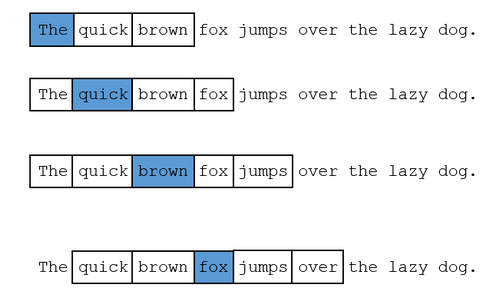
\includegraphics[width=0.5\columnwidth]{./Figures/window.png} % Example image
	\caption{Janela de contexto se movimentando com as iterações do algoritmo.}
\end{figure}

O tamanho da janela de contexto foi variado entre o conjunto de valores \textbf{5}, \textbf{10}, \textbf{15} e \textbf{20}.
O código do \texttt{Word2Vec} também possui funções de \textit{negative sampling} e \textit{hierarchical softmax}. Esses parâmetros não foram variados e o seu funcionamento não será abordado nesse trabalho. Os dois parâmetros assim como os demais foram mantidos os mesmos que vem de padrão com o código, com exceção dos parâmetros de tamanho da janela de contexto e se o algoritmo deve usar o CBOW ou o skip-gram.


\section{Resultados}

O conjunto de hiper-parâmetros apresentados na Seção \ref{sec:hiperparams} define 32 modelos de linguagem distintos. Os modelos foram treinados e avaliados de acordo com a distância do cosseno.
Os resultados obtidos estão na Figura \ref{fig:results}:

\begin{figure}[H]\label{fig:results} % [h] forces the figure to be output where it is defined in the code (it suppresses floating)
	\centering
	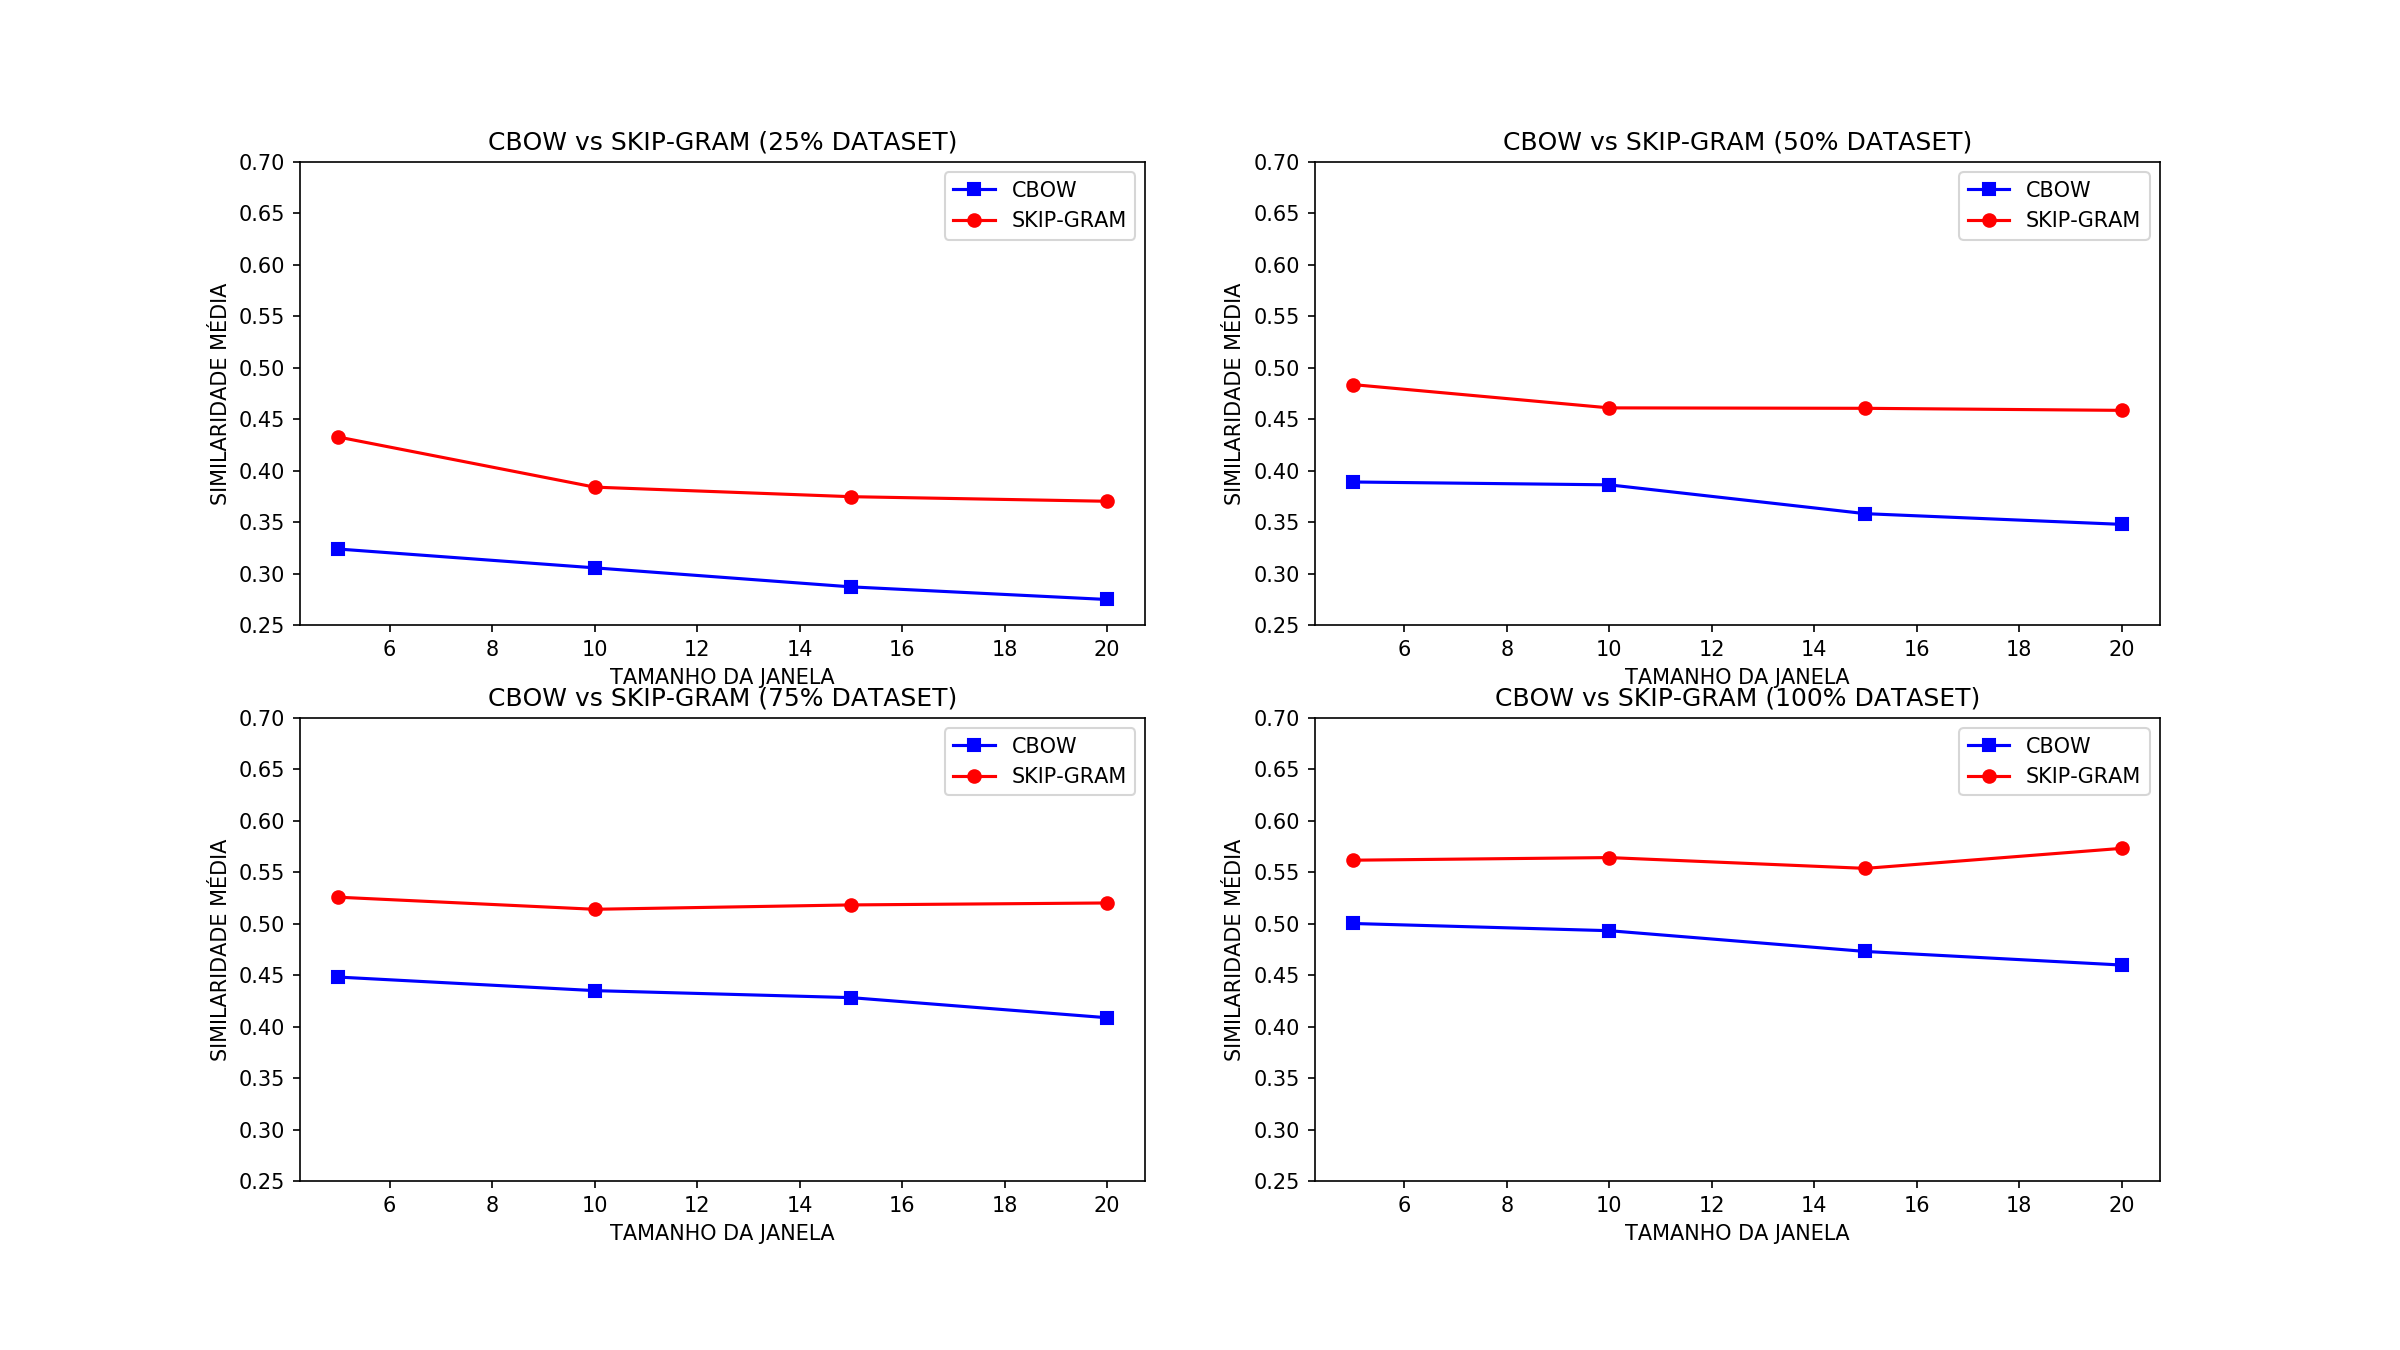
\includegraphics[width=1\columnwidth]{./Figures/results.png} % Example image
	\caption{Resultados obtidos para o conjunto de 32 modelos \texttt{Word2Vec}.}
\end{figure}
A distância do cosseno é uma medida de similaridade e quanto maior seu valor, mais similar dois vetores são.

A partir da Figura \ref{fig:results} é possível visualizar que a abordagem usando o \texttt{skip-gram} forneceu, em média, respostas mais similares ao resultado correto em relação ao \texttt{CBOW}. Também observa-se que aumentar o tamanho do conjunto de dados melhorou o desempenho dos modelos, independentemente do tamanho da janela escolhida.

\section{Conclusões}

Nesse trabalho foi possível estudar o modelo de linguagem \textit{Word2Vec} e entender melhor seu funcionamento. O aluno se familiarizou com a implementação fornecida pelo professor e apresentou uma rotina de avaliação do algoritmo ao variar os parâmetros especificados.

Os resultados obtidos foram coerentes e esperados, o modelo \texttt{skip-gram} geralmente se comporta melhor que o \texttt{CBOW} em datasets pequenos como o utilizado. A melhora nos resultados com o aumento do conjunto de treinamento também é coerente, pois existe mais contexto para os modelos aprenderem e generalizar melhor.


\section{Referências}

1 - Notas de Aula do Professor Adriano Veloso, disciplina de Aprendizado Profundo para Processamento de Linguagem Natural.

2 - \hyperlink{https://israelg99.github.io/2017-03-23-Word2Vec-Explained/}{https://israelg99.github.io/2017-03-23-Word2Vec-Explained/}

\end{document}
